\chapter{Chess}
\label{ch:chess_app}
In this appendix, we briefly discuss the rules of chess together with some notions used throughout the main content of the dissertation. It is only advised to those without game specific knowledge to read this chapter. First, we summarize the rules in section \ref{sec:rules}. Chess players can be classified in strength with a rating system laid out in section \ref{sec:elo}. To finalize, some chess specific terms used in the thesis are defined in \ref{sec:chessjargon}.

\section{Rules}
\label{sec:rules}
Chess is a game played with two players denoted by the color of their pieces: black and white. Both sides start with 16 pieces at the start of the game. The players are allowed to play one move with one of their pieces on a checkered board every turn. Every square on this board has its own unique name as denoted in figure \ref{fig:empty}. The allowed movements on the chessboard are further discussed in section \ref{subsec:cp}. The ultimate goal of both sides is to checkmate the opponent, which is explained in section \ref{subsec:cp}. Only the most noteworthy game specific elements are explained in this section, an official and complete explanation is provided by the FIDE (the world chess federation) \cite{ruleschess}.

\begin{figure}
\centering
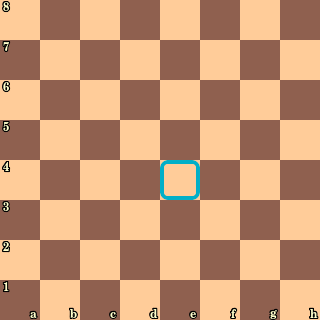
\includegraphics[scale=0.5]{fig/rules/empty}
\caption[Chessboard layout]{The chessboard layout. The rows and columns are identified with letters and numbers respectively. For example, the marked square is e4.}
\label{fig:empty}
\end{figure}

\subsection{Chess Pieces}
\label{subsec:cp}
Every piece is allowed to take other pieces from the opponent, but is blocked by its own kind.
The mobility of every piece is indicated in figure \ref{fig:pm}. During the game, some special moves may occur, these are explained in section \ref{subsec:special_mvs} The initial setup of the board is depicted in figure \ref{fig:initial}.

\begin{figure}
    \centering
    \begin{subfigure}[b]{0.4\textwidth}
        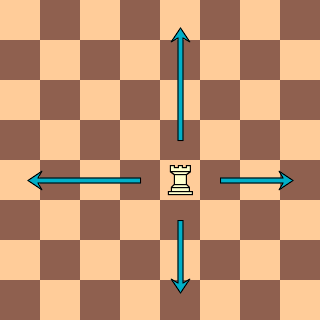
\includegraphics[scale=0.5]{fig/rules/rook}
        \caption{Rook}
        \label{fig:rook}
    \end{subfigure}
    \qquad
    \begin{subfigure}[b]{0.4\textwidth}
         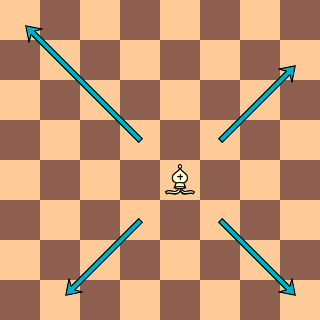
\includegraphics[scale=0.5]{fig/rules/bishop}
        \caption{Bishop}
        \label{fig:bishop}
    \end{subfigure}
    \\
    \begin{subfigure}[b]{0.4\textwidth}
        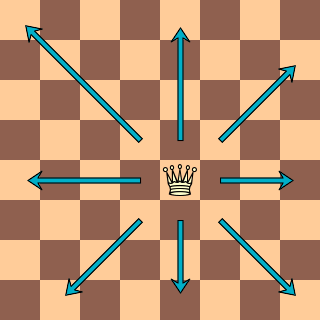
\includegraphics[scale=0.5]{fig/rules/queen}
        \caption{queen}
        \label{fig:queen}
    \end{subfigure}
    \qquad
    \begin{subfigure}[b]{0.4\textwidth}
         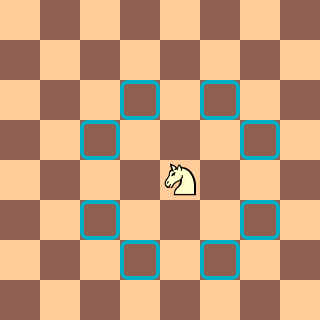
\includegraphics[scale=0.5]{fig/rules/knight}
        \caption{knight}
        \label{fig:knight}
    \end{subfigure}
    \\
    \begin{subfigure}[b]{0.4\textwidth}
            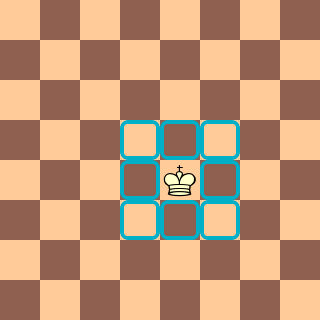
\includegraphics[scale=0.5]{fig/rules/king}
            \caption{king}
            \label{fig:king}
        \end{subfigure}
        \qquad
        \begin{subfigure}[b]{0.4\textwidth}
             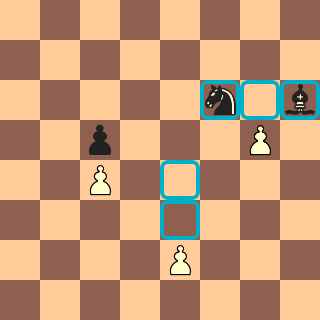
\includegraphics[scale=0.5]{fig/rules/pawn}
            \caption{pawn}
            \label{fig:pawn}
        \end{subfigure}
        \caption[Piece mobility]{Piece mobility. (a) The rook is allowed to move vertically and horizontally. (b) The bishop can move diagonally. (c) The queen's mobility is the combination of the rook's and bishop's. (d) The knight is the only piece that can 'jump' over pieces, by moving in an L-structure. (e) The king's movement is the same as the queen's, but is limited to the surrounding squares. (f) The pawn moves one square forward, but can only capture diagonally. When it is at its starting position (see figure ), it can travel 2 squares forward as well.}
        \label{fig:pm}

\end{figure}

\begin{figure}
\centering
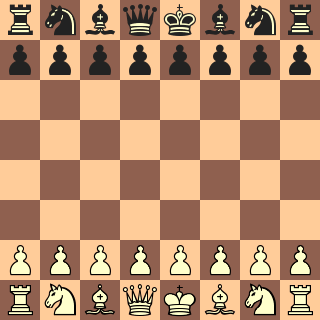
\includegraphics[scale=0.5]{fig/rules/initial}
\caption[Chess starting position]{The initial set up of chess. White is the first side to make a move.}
\label{fig:initial}
\end{figure}

\subsection{Special Positions}
\label{subsec:special_pos}
During a game of chess, some special positions may occur. Some examples are demonstrated in figure \ref{fig:pos} to clear things up.
\begin{itemize}
\item \textbf{check.} The king is under attack, an opponent's piece would capture the king if it were not to move. The rules of chess prohibit the possibility of a king being captured. To this reason, the player is obliged to make a move escaping the assault on the king.
\item \textbf{checkmate.} This is a check where no legal move can be played. This ends the game in favor of the player performing the checkmate.
\item \textbf{stalemate.} There are no legal moves left, but the king is not under attack. These positions are followed by a draw (see section \ref{subsec:termination}).
\end{itemize}

\begin{figure}
    \centering
    \begin{subfigure}[b]{0.4\textwidth}
        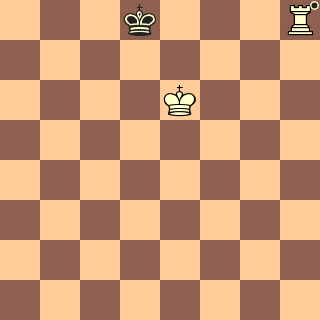
\includegraphics[scale=0.5]{fig/rules/check1}
        \caption{Example of check}
        \label{fig:check1}
    \end{subfigure}
    \qquad
    \begin{subfigure}[b]{0.4\textwidth}
         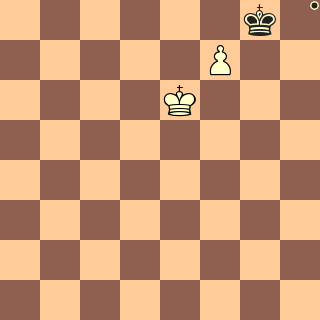
\includegraphics[scale=0.5]{fig/rules/check2}
        \caption{Example of check}
        \label{fig:check2}
    \end{subfigure}
    \\
    \begin{subfigure}[b]{0.4\textwidth}
        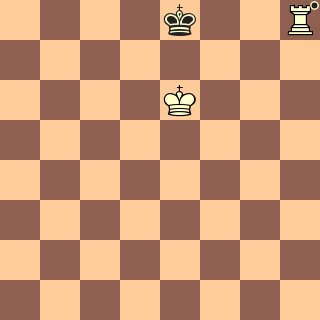
\includegraphics[scale=0.5]{fig/rules/mate1}
        \caption{Example of checkmate}
        \label{fig:mate1}
    \end{subfigure}
    \qquad
    \begin{subfigure}[b]{0.4\textwidth}
         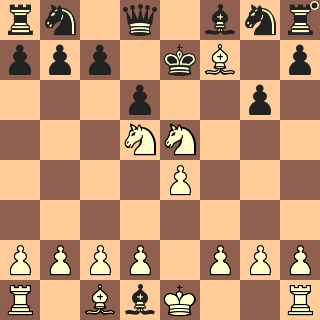
\includegraphics[scale=0.5]{fig/rules/mate_2}
        \caption{\textit{Legall}'s checkmate}
        \label{fig:mate2}
    \end{subfigure}
    \\
    \begin{subfigure}[b]{0.4\textwidth}
            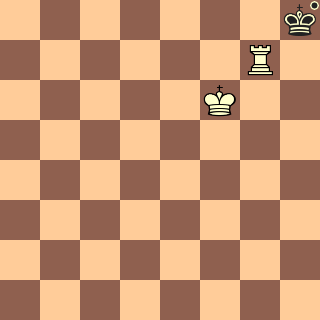
\includegraphics[scale=0.5]{fig/rules/stalemate1}
            \caption{Example of stalemate}
            \label{fig:stalemate1}
        \end{subfigure}
        \qquad
        \begin{subfigure}[b]{0.4\textwidth}
             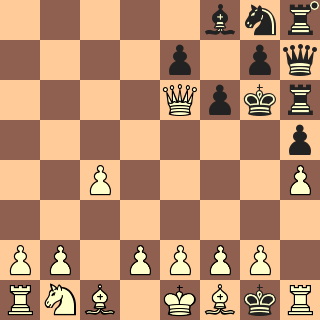
\includegraphics[scale=0.5]{fig/rules/stalemate2}
            \caption{Example of stalemate}
            \label{fig:stalemate2}
        \end{subfigure}
        \caption{Special chess positions}
        \label{fig:pos}

\end{figure}

\subsection{Special Moves}
\label{subsec:special_mvs}
There exist three special moves, which happen rarely during a game of chess.
\begin{itemize}
\item \textbf{castling.} When the king and rook have not been moved yet during the game, castling may occur. This consists of moving the king two squares towards a rook at the base rank as indicated in figure \ref{fig:castle}, followed by placing the rook next to the king at the opposite side of the king movement. 
\item \textbf{en passant capture.} To make up for the double push of pawns at their starting positions and hence missed opportunity for their adversed counterparts, pawns at the fourth rank have one and only one chance to capture these double pushed pawns.
\item \textbf{promotion.} When a pawn reaches the last rank (thus it would not be able to move forward anymore), it gets promoted to one of the following pieces: queen, rook, bishop, knight. A queen promotion is shown in figure \ref{fig:prom}.
\end{itemize}

\begin{figure}
\centering
\begin{subfigure}[b]{0.4\textwidth}
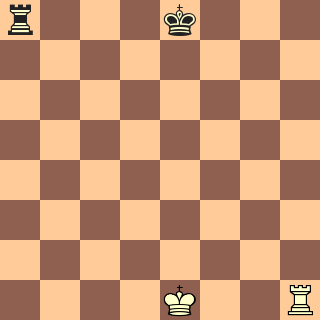
\includegraphics[scale=0.5]{fig/rules/castle_before}
\caption{before castling}
\label{fig:castle_bef}
\end{subfigure}
\qquad
\begin{subfigure}[b]{0.4\textwidth}
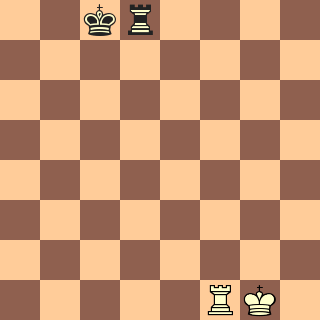
\includegraphics[scale=0.5]{fig/rules/castle_after}
\caption{after castling}
\label{fig:castle_aft}
\end{subfigure}
\qquad
\begin{subfigure}[b]{0.4\textwidth}
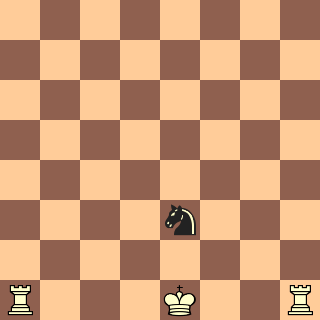
\includegraphics[scale=0.5]{fig/rules/castle_no}
\caption{castling is not allowed}
\end{subfigure}
\caption[Castling]{(a) \& (b): White performs king side castling, while black castles queen side. (c) Castling is forbidden in case the king had to pass an attacked square (Here squares f1 and d1 for king side and queen side castling respectively).}
\label{fig:castle}
\end{figure}

\begin{figure}
\centering
\begin{subfigure}[b]{0.4\textwidth}
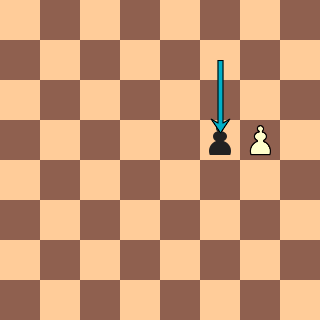
\includegraphics[scale=0.5]{fig/rules/ep_before}
\caption{Before en passant capture}
\label{fig:ep_bef}
\end{subfigure}
\qquad
\begin{subfigure}[b]{0.4\textwidth}
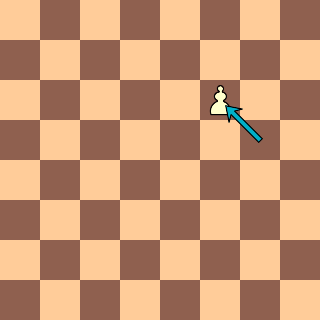
\includegraphics[scale=0.5]{fig/rules/ep_after}
\caption{After en passant capture}
\end{subfigure}
\caption[En passant capture]{Demonstration of how an en passant move is performed.}
\label{fig:ep}
\end{figure}

\begin{figure}
\centering
\begin{subfigure}[b]{0.4\textwidth}
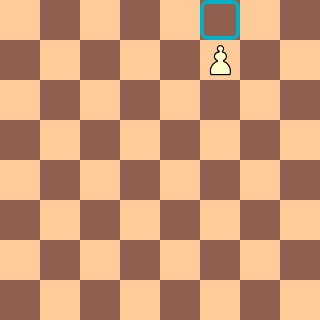
\includegraphics[scale=0.5]{fig/rules/promotion_before}
\caption{Before queen promotion}
\end{subfigure}
\qquad
\begin{subfigure}[b]{0.4\textwidth}
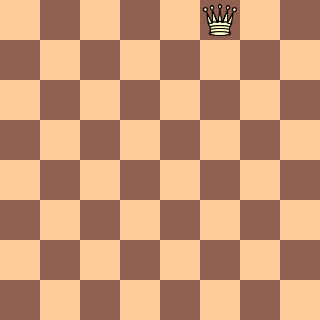
\includegraphics[scale=0.5]{fig/rules/promotion_after}
\caption{After queen promotion}
\end{subfigure}
\caption[Promotion]{Promotion of a pawn to a queen.}
\label{fig:prom}
\end{figure}

\subsection{Termination}
\label{subsec:termination}
There are three possible results to a chess game:
\begin{enumerate}
\item white wins: 1-0
\item draw: 1/2-1/2
\item black wins: 0-1
\end{enumerate}
The game terminates when one of the following events occur:
\begin{itemize}
\item checkmate, wins the game.
\item a player resigns, hence he loses.
\item stalemate results in a draw
\item insufficient mating material, when it is impossible to achieve a checkmate through legal play the game is drawn.
\item draw by agreement
\item draw by repetition can be claimed after reaching the exact same board position three times over the course of the game
\item 50-move rule, when no opponent is making any progress, a draw can be claimed. This is defined as 50 moves (both black and white) without any captures and pawn moves.
\end{itemize}
It may be interesting to note that the rules of chess are designed in such a way that every game would end eventually.

\section{Evaluation of Strength}
\label{sec:elo}
To assess the strength of chess players, the \textit{Elo} rating system has been invented by Hungarian physicist \textit{Arpad Elo}. It has been used as a competitive score since then for other games like scrabble. The idea is to use the rating difference as a predictor of the match. Based on the probabilistic prediction and the true outcome, the players' ratings are adjusted. This means that winning against a stronger opponent results is a higher elo gain and vice versa.\\

Suppose player $A$ with rating $R_A$ plays against player $B$ with rating $R_B$. The expected outcome of the game with respect to $A$ is then
\[
E_A=\frac{Q_A}{Q_A+Q_B}
\]
with
\begin{align*}
Q_A&=10^{R_A/400} \\
Q_B&=10^{R_B/400}
\end{align*}
Hence the outcome is estimated with a logistic curve with base 10. This means that every rating difference of 400 points estimates the ratio of outcomes 10:1 in favor of the highest rating. The effective outcomes can be
\begin{equation*}
S_A = \begin{cases} 
   1 & $A$ \text{ wins} \\
   \frac{1}{2} & \text{draw} \\
   0 & $A$ \text{ loses} \\
  \end{cases}
\end{equation*}
The rating of $A$ is then updated with
\[
R_A\leftarrow R_A+K(S_A-E_A)
\]
with $K$ being the $K$-factor. In FIDE regulations, $K$ gets smaller after playing more matches and achieving a higher rating, as the uncertainty about the real strength has decreased.

\section{Chess Jargon}
\label{sec:chessjargon}
Chess specific words that may be beneficial for understanding certain concepts within this document are presented in table \ref{tab:gls}.

\begin{table}[]
\centering
\caption{Glossary with chess terms}
\label{tab:gls}
\begin{tabular}{rL{10cm}}
\hline
\textbf{attack}       & a piece is under attack if there is a direct threat to capture it \\ \hline
\textbf{black}        & player of the black pieces                                       \\ \hline
\textbf{board}        & chessboard      \\                                                  \hline
\textbf{capture}      & a piece moves to a square occupied by the opponent              \\  \hline
\textbf{castling}     &  see section \ref{subsec:special_mvs}                                                                 \\ \hline
\textbf{check}        & see section \ref{subsec:special_mvs}                                                                  \\ \hline
\textbf{checkmate}    &   see section \ref{subsec:special_mvs}                                                                                                     \\\hline
\textbf{draw}         &  see section \ref{subsec:termination}                                                                 \\ \hline
\textbf{endgame}      &  the last phase possible in a chess game, where most pieces have already \newline been captured.                                                               \\ \hline
\textbf{en passant}   & see section \ref{subsec:special_mvs}                                                                  \\ \hline
\textbf{exchange}     & an exchange denotes the balance between the captured pieces of both sides in a move sequence                                                                  \\ \hline
\textbf{file}        &  vertical set of squares on the board                                                                \\ \hline
\textbf{half move}  &  one ply \\ \hline
\textbf{kingside}     &  the right half of the board (in white's perspective)                                                                 \\ \hline
\textbf{mate}         &  same as checkmate                                                                 \\ \hline
\textbf{middle game}  &   stage of the game between the opening and endgame                                                               \\ \hline
\textbf{minor piece}  &  a bishop or a knight
\\ \hline
\textbf{move}  & Depending on the context one or two plies or half moves.                                                   \\ \hline
\textbf{opening}      &  the first phase of the game, when most of the pieces are still on the board. More or less the first                                                                  \\ \hline
\textbf{piece}        & One of the 32 figurines of the game                                                                  \\ \hline
\textbf{promotion}    & see section \ref{subsec:special_mvs}                                                                  \\
\textbf{queenside}    & the left half of the board (in white's perspective)                                                                   \\ \hline
\textbf{rank}         & a row, generally denoted by a number from 1 to 8                                                                  \\ \hline
\textbf{repetition}   &  see section \ref{subsec:termination}                                                                 \\ \hline
\textbf{stalemate}    & see section \ref{subsec:special_pos}                                                                  \\ \hline
\textbf{white}        & player of the white pieces                                                                  \\ \hline
\textbf{50 move rule} &  see section \ref{subsec:termination}          \\                                                      \hline
\end{tabular}
\end{table}